\documentclass{article}
\usepackage{graphicx} % Required for inserting images
\usepackage{tikz}
\usepackage{chemfig}
\usepackage{mhchem}
\usepackage{amsmath}

\title{NOx Cycle}
\author{Samuel Arnold}
\date{Last Modified: October 2026}

\begin{document}

\maketitle

\section*{LNOx Cycle}

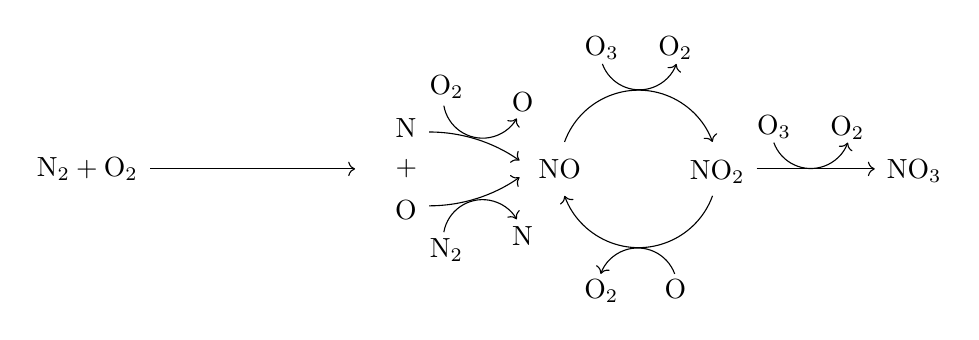
\begin{tikzpicture}[->,scale=1]
    %Creates all of the nodes and locations
    % \node (Name) at (angle:radius) {equation/visible label};
    \node (N2/O2) at (180:7cm) {$\ce{N2 + O2}$};
    \node (N) at (170:3cm) {$\ce{N}$};
    \node (+) at (180:2.95cm) {$\ce{+}$};
    \node (O) at (190:3cm) {$\ce{O}$};
    \node (O2) at (157:2.65cm) {$\ce{O2}$};
    \node (O) at (150:1.7cm) {$\ce{O}$};
    \node (N2) at (203:2.65cm) {$\ce{N2}$};
    \node (N) at (210:1.7cm) {$\ce{N}$};
    \node (NO) at (180:1cm) {$\ce{NO}$};
    \node (O3) at (107:1.6cm) {$\ce{O3}$};
    \node (O2) at (73:1.6cm) {$\ce{O2}$};
    \node (NO2) at (-2:1cm) {$\ce{NO2}$};
    \node (O2) at (253:1.62cm) {$\ce{O2}$};
    \node (O) at (287:1.6cm) {$\ce{O}$};
    \node (NO3) at (-0.5:3.5cm) {$\ce{NO3}$};
    \node (O3) at (17:1.8cm) {$\ce{O3}$};
    \node (O2) at (11:2.7cm) {$\ce{O2}$};
    
    %--------------------------------------------------------------------------------------
    %Creates the lines connecting the nodes, done in polar coordinates essentially
    % \draw (angleStart:radiusStart) to (angleEnd:radiusEnd);   %for line
    % \draw (angleStart:radiusStart) arc (arcAngleStart:arcAngleEnd:arcRadius);   %for arcs
    \draw (180:6.2cm) to (180:3.6cm); %N2+O2 to N+O line
    \draw (170:2.7cm) arc (90:55:2cm); %N to NO arc
    \draw (190:2.7cm) arc (-90:-55:2cm); %O to NO arc
    \draw (162:2.6cm) arc (190:330:0.5cm); %O2 to O arc
    \draw (198:2.6cm) arc (-190:-330:0.5cm); %N2 to N arc
    \draw (160:1cm) arc (160:20:1cm); %NO to NO2 arc
    \draw (109:1.41cm) arc (-160:-20:0.5cm); %O3 to O2 arc
    \draw (-20:1cm) arc (-20:-160:1cm); %NO2 to NO arc
    \draw (289:1.41cm) arc (20:160:0.5cm); %O to O2 arc
    \draw (0:1.5cm) to (0:3cm); %NO2 to NO3 line
    \draw (11:1.75cm) arc (-160:-20:0.5cm); %O3 to O2 arc

\end{tikzpicture}

\section*{Rocket Emissions NOx Cycle}

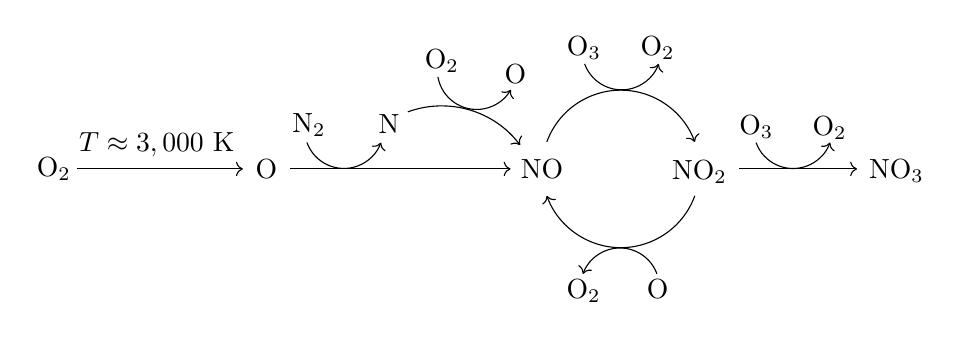
\begin{tikzpicture}[->,scale=1]
    %Creates all of the nodes and locations
    % \node (Name) at (angle:radius) {equation/visible label};
    \node (O2_dissoc) at (180:7.2cm) {$\ce{O2}$};
    \node (heat) at (177: 5.9cm) {$T \approx 3,000$ K};
    \node (O) at (180:4.5cm) {$\ce{O}$};
    \node (N) at (169:3cm) {$\ce{N}$};
    \node (N2) at (172:4cm) {$\ce{N2}$};
    \node (O2) at (149:2.65cm) {$\ce{O2}$};
    \node (O) at (138:1.8cm) {$\ce{O}$};
    \node (NO) at (180:1cm) {$\ce{NO}$};
    \node (O3) at (107:1.6cm) {$\ce{O3}$};
    \node (O2) at (73:1.6cm) {$\ce{O2}$};
    \node (NO2) at (-2:1cm) {$\ce{NO2}$};
    \node (O2) at (253:1.62cm) {$\ce{O2}$};
    \node (O) at (287:1.6cm) {$\ce{O}$};
    \node (NO3) at (-0.5:3.5cm) {$\ce{NO3}$};
    \node (O3) at (17:1.8cm) {$\ce{O3}$};
    \node (O2) at (11:2.7cm) {$\ce{O2}$};
    
    %--------------------------------------------------------------------------------------
    %Creates the lines connecting the nodes, done in polar coordinates essentially
    % \draw (angleStart:radiusStart) to (angleEnd:radiusEnd);   %for line
    % \draw (angleStart:radiusStart) arc (arcAngleStart:arcAngleEnd:arcRadius);   %for arcs
    \draw (180:6.9cm) to (180:4.8cm); %O2 to O line
    \draw (165:2.8cm) arc (110:37:1.25cm); %N to NO arc
    \draw (180:4.2cm) to (180:1.4cm); %O to NO line
    \draw (175.2:4cm) arc (-160:-20:0.5cm); %N2 to N arc
    \draw (153.3:2.6cm) arc (190:330:0.5cm); %O2 to O arc
    \draw (160:1cm) arc (160:20:1cm); %NO to NO2 arc
    \draw (109:1.41cm) arc (-160:-20:0.5cm); %O3 to O2 arc
    \draw (-20:1cm) arc (-20:-160:1cm); %NO2 to NO arc
    \draw (289:1.41cm) arc (20:160:0.5cm); %O to O2 arc
    \draw (0:1.5cm) to (0:3cm); %NO2 to NO3 line
    \draw (11:1.75cm) arc (-160:-20:0.5cm); %O3 to O2 arc

\end{tikzpicture}




\end{document}
